% bei Standalone in documentclass noch:
% \RequirePackage{luatex85}

\documentclass[captions=tableheading, titlepage= firstiscover, parskip = half , bibliography=totoc]{scrartcl}
%paper = a5 fÃŒr andere optinen
% titlepage= firstiscover
% bibliography=totoc fÃŒr bibdateien
% parskip=half  VerÀnderung um AbsÀtze zu verbessern

\usepackage{scrhack} % nach \documentclass
\usepackage[aux]{rerunfilecheck}
\usepackage{polyglossia}
\usepackage[style=numeric, backend=biber]{biblatex} % mit [style = alphabetic oder numeric] nach polyglossia
\addbibresource{lit.bib}
\setmainlanguage{german}

\usepackage[autostyle]{csquotes}
\usepackage{amsmath} % unverzichtbare Mathe-Befehle
\usepackage{amssymb} % viele Mathe-Symbole
\usepackage{mathtools} % Erweiterungen fÃŒr amsmath
\usepackage{fontspec} % nach amssymb
% muss ins document: \usefonttheme{professionalfonts} % fÌr Beamer PrÀsentationen
\usepackage{longtable}
\usepackage{dsfont}
\usepackage[
math-style=ISO,    % \
bold-style=ISO,    % |
sans-style=italic, % | ISO-Standard folgen
nabla=upright,     % |
partial=upright,   % /
]{unicode-math} % "Does exactly what it says on the tin."
\setmathfont{Latin Modern Math}
% \setmathfont{Tex Gyre Pagella Math} % alternativ

\usepackage[
% die folgenden 3 nur einschalten bei documenten
locale=DE,
separate-uncertainty=true, % Immer Fehler mit ±
per-mode=symbol-or-fraction, % m/s im Text, sonst \frac
]{siunitx}

% alternativ:
% per-mode=reciprocal, % m s^{-1}
% output-decimal-marker=., % . statt , fÃŒr Dezimalzahlen

\usepackage[
version=4,
math-greek=default,
text-greek=default,
]{mhchem}

\usepackage[section, below]{placeins}
\usepackage{caption} % Captions schöner machen
\usepackage{graphicx}
\usepackage{grffile}
\usepackage{subcaption}

% \usepackage{showframe} Wenn man die Ramen sehen will

\usepackage{float}
\floatplacement{figure}{htbp}
\floatplacement{table}{htbp}

\usepackage{mathtools}

\usepackage{booktabs}

 \usepackage{microtype}
 \usepackage{xfrac}

 \usepackage{expl3}
 \usepackage{xparse}

 % \ExplSyntaxOn
 % \NewDocumentComman \I {}  %Befehl\I definieren, keine Argumente
 % {
 %    \symup{i}              %Ergebnis von \I
 % }
 % \ExplSyntaxOff

 \usepackage{pdflscape}
 \usepackage{mleftright}

 % Mit dem mathtools-Befehl \DeclarePairedDelimiter können Befehle erzeugen werden,
 % die Symbole um AusdrÃŒcke setzen.
 % \DeclarePairedDelimiter{\abs}{\lvert}{\rvert}
 % \DeclarePairedDelimiter{\norm}{\lVert}{\rVert}
 % in Mathe:
 %\abs{x} \abs*{\frac{1}{x}}
 %\norm{\symbf{y}}

 % FÃŒr Physik IV und Quantenmechanik
 \DeclarePairedDelimiter{\bra}{\langle}{\rvert}
 \DeclarePairedDelimiter{\ket}{\lvert}{\rangle}
 % <name> <#arguments> <left> <right> <body>
 \DeclarePairedDelimiterX{\braket}[2]{\langle}{\rangle}{
 #1 \delimsize| #2
 }

\setlength{\delimitershortfall}{-1sp}

 \usepackage{tikz}
 \usepackage{tikz-feynman}

 \usepackage{csvsimple}
 % Tabellen mit \csvautobooktabular{"file"}
 % muss in table umgebung gesetzt werden


% \multicolumn{#Spalten}{Ausrichtung}{Inhalt}

\usepackage{hyperref}
\usepackage{bookmark}
\usepackage[shortcuts]{extdash} %nach hyperref, bookmark

\newcommand{\ua}[1]{_\symup{#1}}
\newcommand{\su}[1]{\symup{#1}}

\begin{document}
\section{Zielsetzung}
In diesem Versuch sollen für die Rubidium-Isotope $^{85}\su{Rb}$ und $^{87}\su{Rb}$ die Landé-Faktoren und
daraus folgenden Spins der Elektronenhülle und des Kernspins mittels des optischen Pumpens bestimmt werden.
\section{Theorie}
vollständig mit Elektronen besetzt. Bei äußeren Energieniveaus hingegen kommt es
zur temperaturabhängigen Besetzung. Diese wird durch die Boltzmannsche Gleichung
\begin{align}
    \frac{N_{2}}{N_{1}} = \frac{g_{2}}{g_{1}}\frac{\exp(-W_{2}/\su{kT})}{\exp(-W_{1}/\su{kT})}
    \label{eqn:boltzmann}
\end{align}
mit den Zuständen $N_1$, $N_2$ und den Energien $W_1$, $W_2$
beschreiben. Die statistischen Gewichte $g_i$ geben die Anzahl der zu der Energie
$W_i$ gehörigen Zustände an.
Durch das optische Pumpen ist es möglich die in \ref{eqn:boltzmann} gegebene Verteilung
zu verändern bis zu einer Inversion der Besetzungszustände mit $N_2 > N_1$.
Diese Inversion können dann zur Induzierung von Strahlungsübergängen verwendet werden.
Die Energiedifferenz
\begin{align*}
    h\nu = W_{2}-W_{1}
\end{align*}
kann für kleine Energien mithilfe der Hyperfeinstrukturaufspaltung und
Zeeman-Aufspaltung präzise bestimmt werden.

\subsection{Zeeman-Effekt}
In der ersten Näherung wird davon ausgegangen, dass die beiden Rubidium-Isotope einen verschwindenen
Kernspin besitzen. Der Gesamtdrehimpuls der Elektronenhülle $\vec{J}$ koppelt an ein
magnetisches Moment $\vec{\mu_{\su{J}}}$, was durch
\begin{align*}
    \vec{\mu_{\su{j}}} &= -g_{\su{j}} \mu_{\su{B}} \vec{J} \\
    |\vec{\mu_{\su{j}}}| &= g_{\su{j}} \mu_{\su{B}} \sqrt{J(J+1)}
\end{align*}
beschrieben wird. Dabei ist $\mu_{\su{B}}$ das Bohrsche Magneton, $g_{\su{J}}$ der Landé-Faktor, welcher
die Zusammensetzung des magnetischen Moments aus Bahndrehimpuls $\vec{L}$ und Spin $\vec{S}$ berücksichtigt.
Es folgt für das Gesamtmoment
\begin{align*}
    \vec{\mu_{\su{J}}} = \vec{\mu_{\su{L}}} + \vec{\mu_{\su{S}}}.
\end{align*}
Beim Anlegen eines Magnetfeldes B kommt es zur Energieaniveauaufspaltung in $2J+1$ Unterniveaus
\begin{align*}
    U_{\su{magn}} = M_{\su{J}} g_{\su{J}} \mu_{\su{B}} \su{B}.
\end{align*}
Diese Niveaufspaltung wird als Zeeman-Effekt bezeichnet.

\subsection{Hyperfeinstrukturaufspaltung}
Da die Rubidium-Isotope keinen verschwindenden Kernspin besitzen, muss die Hyperfeinstruktur der
einzelnen Energieniveaus und der daraus folgende Einfluss auf die Zeeman-Aufspaltung berücksichtigt werden.
Der Kernspin $\vec{I}$ koppelt dann mit dem Gesamtdrehimpuls des Elektronenhülle $\vec{J}$ zum Gesamtdrehimpuls
des Atoms
\begin{align*}
    \vec{F} = \vec{J} + \vec{I}.
\end{align*}
Die Quantenzahl F kann die Werte von $I+J$ bis $|I-J|$ annehmen und folglich die Hyperfeinstrukturterme für den ersten Fall mit $J<I$: $2J+1$, und für den zweiten Fall mit
$J>I$: $2I+1$.
Durch das Anlegen eines äußeren Magnetfeldes kommt es zur weiteren Aufspaltung der Hyperfeinstrukturterme
in $2F+1$-Zeeman-Niveaus. Die Energiedifferenz zweier benachbarter Niveaus folgt aus
\begin{align*}
    U_{\symup{HF}} = g_{\symup{F}} \mu_{\symup{B}} B.
\end{align*}
Der Landé-Faktor $g_{\symup{F}}$ folgt aus der vektoriellen Betrachtung
\begin{align*}
    g_{\su{F}} \approx g_{\su{J}} \frac{F(F+1)+J(J+1)-I(I+1)}{2F(F+1)}.
\end{align*}
Dies ist für ein Alkali Atom mit $J=\frac{1}{2}$ und $I=\frac{3}{2}$ beispielhaft in Abbildung \ref{fig:alkali}
dargestellt.
\begin{figure}
    \centering
    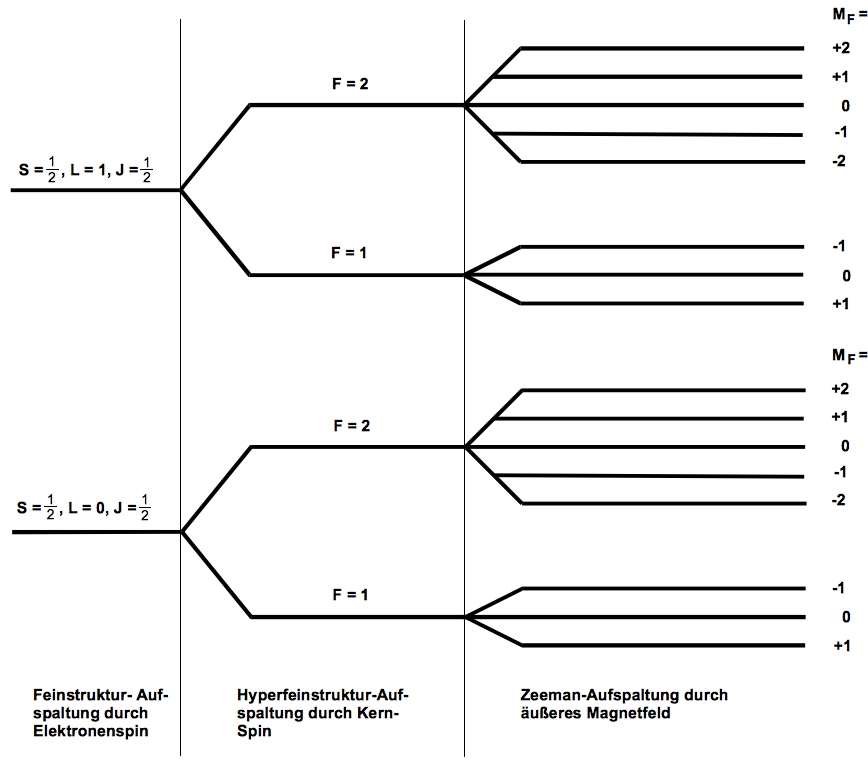
\includegraphics[scale = 0.54]{pictures/alkali.png}
    \caption{Hyperfeinstruktur- und Zeeman-Aufspaltung für einen $L=0$- und $L=1$-Zustand.\cite{1}}
    \label{fig:alkali}
\end{figure}

\subsection{Optische Pumpen}
Der Übergang in ein anderes Niveau kann nur unter Berücksichtigung der Auswahlregeln
$\Delta M_{\su{J}} = 0, \pm1$ erfolgen. Diese Übergänge unterschieden sich in ihrer Energie
und Polarisation.
Der $\sigma^{+}$-Übergang mit $\Delta M_{\text{J}} = 1$ kann nur mit rechszirkular-polarisierten Licht hervorgerufen werden,
wohingegen der $\sigma^{-}$-Übergang mit $\Delta M_{\text{J}} = -1$
Diese beiden Übergänge emittieren zirkular-polarisiertes Licht in Magnetfeldrichtung, in den dazu senkrecht
Richtung.
Der $\pi$-Übergang mit $\Delta M_{\text{J}} = 0$ emittiert parallel zum Magnetfeld linear polarisiertes
Licht. \newline
Die Zeeman-Aufspaltun mit den unterschiedlichen Übergängen und unter Vernachlässigung des Kernspins ist in Abbildung \ref{fig:übergänge}
für eine hypothetisches Alkali-Atom dargestellt.
\begin{figure}
    \centering
    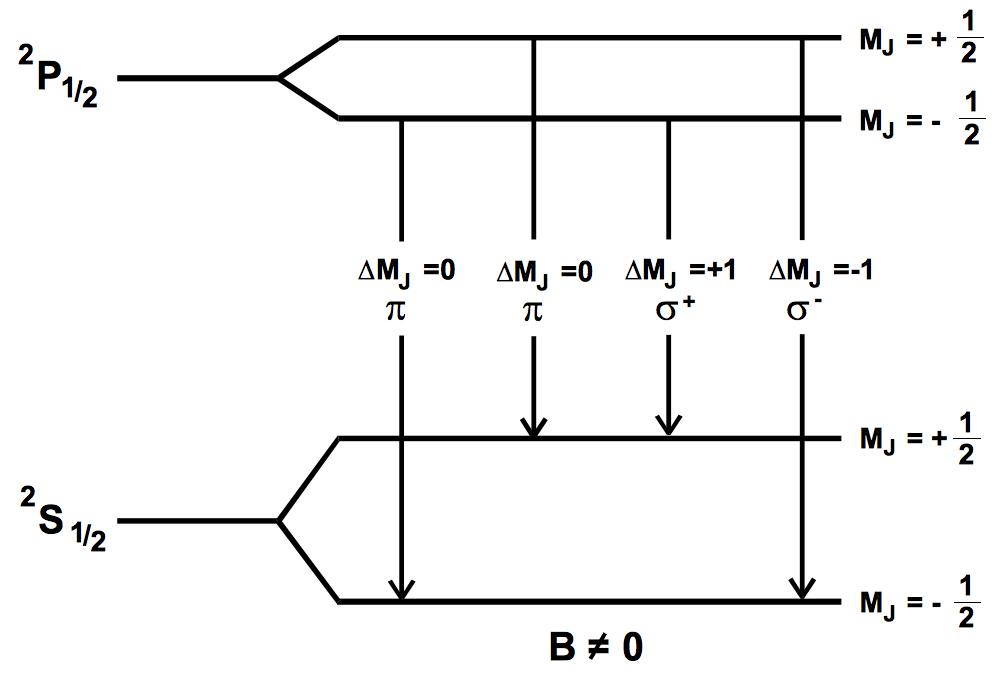
\includegraphics[scale = 0.38]{pictures/übergänge.png}
    \caption{.\cite{1}}
    \label{fig:übergänge}
\end{figure}

Durch das Einstrahlen von rechtszirkular-polarisierten $D_{\su{1}}$-Licht und das Anlegen eines Magnetfeldes
kann ein aus hypothetisches Alkali-Atomen, welche sich alles im thermischen Gleichgewicht befinden, bestehender Dampf
in einen angeregten Zustand übergehen.
Die möglichen Übergänge für diese Alkali-Atome sind in Abbildung \ref{fig:übergängerechts} zu sehen.
\begin{figure}
    \centering
    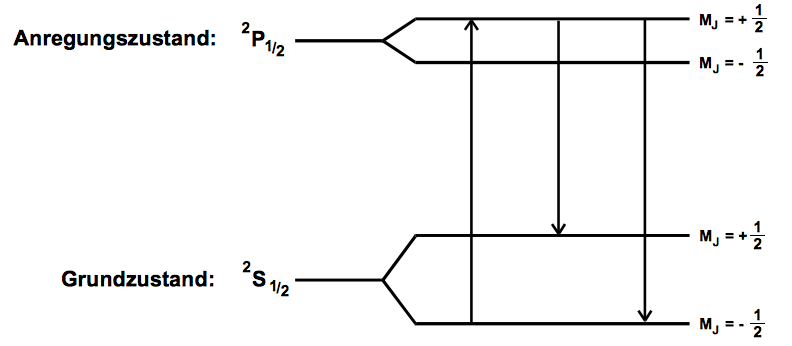
\includegraphics[scale = 0.65]{pictures/übergängerechts.png}
    \caption{Übergangsmöglichkeiten für dieses Beispiel.\cite{1}}
    \label{fig:übergängerechts}
\end{figure}

Die Transparenz der Dampfzelle nimmt zu und läuft asymptotisch gegen 1, wie aus Abbildung \ref{fig:asymptotisch}
\begin{figure}
    \centering
    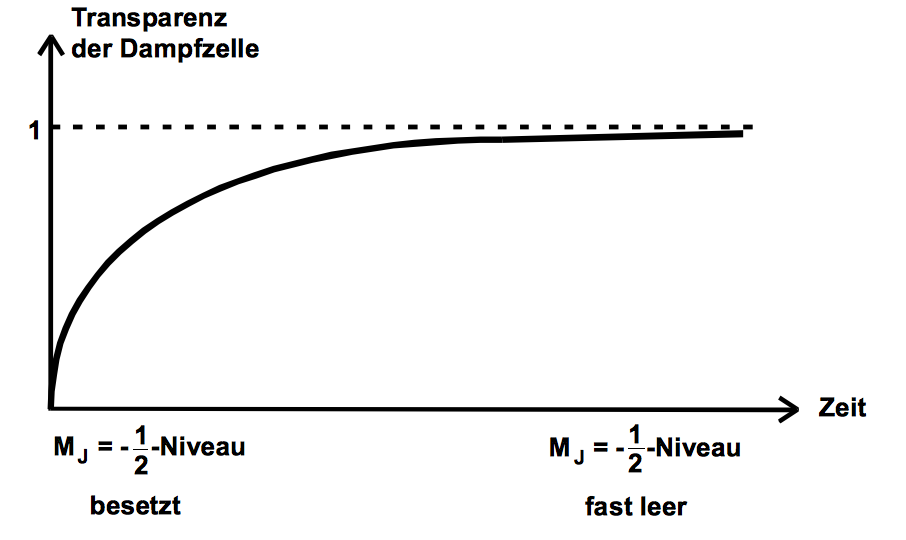
\includegraphics[scale = 0.6]{pictures/asymptotisch.png}
    \caption{Entwicklung der Transparenz unter Einstrahlung des rechtszirkular-polarisierten Liches.\cite{1}}
    \label{fig:asymptotisch}
\end{figure}


\newpage
\subsection{Quadratischer Zeeman-Effekt}
Für größere Magnetfelder können Terme höherer Ordnung nicht vernachlässigt werden.
Durch Lösen der Schrödingergleichung
\begin{align*}
    H \Psi = U \Psi
\end{align*}
mit dem Hamilton-Operator, der sowohl die Spin-Bahn-Wechselwirkung, als auch die Wechselwirkungen
der magnetischen Momente beinhaltet, folgt für die Übergangsenergie
\begin{align*}
     U_{\su{HF}} = g_{\su{F}} \mu{_\su{B}} \su{B} + g_{\su{F}}^2 \mu{_\su{B}}^2 \su{B}^2 \frac{(1-2M_{\su{F}})}{\symup\Delta E_{\su{HF}}} -\,...,
\end{align*}
mit der Energiedifferenz $\Delta E_{\symup{HF}}$ zwischen den Niveaus $F$ und $F+1$.
Somit ist die Zeeman-Energie abhänig von $M_{\symup{F}}$, was als quadratischer Zeeman-Effekt bezeichnet wird.

\subsection{Transiente Effekte}
Bei der Betrachtung von gepumpten Systemen bei denen die Hochfrequenz innerhalb kürzester Zeit ein- und wieder ausgeschaltet wird,
ist die Resonanzfreuqenz gegeben durch
\begin{align*}
    \omega_{\symup{0}} = 2 \pi \nu_{\symup{0}} = g_{\symup{f}} \frac{\nu_{\su{0}}}{h} B_{\su{0}},
\end{align*}
wobei die Larmor-Frequenz durch $\omega_{\su{0}} = \gamma B_{\su{0}}$ mit dem gyromagnetischen Verhältnis
$\gamma = g_{\su{f}} \frac{\mu_{\su{0}}}{h}$ beschrieben wird.
Für den Resonanzfall ergibt sich $B_{\text{RF}} = B_{\text{eff}}$.
\newline
In diesem Fall folgt die Relation
\begin{align*}
    \frac{T_{\su{87}}}{T_{\su{85}}} = \frac{\gamma_{\su{85}}}{\gamma_{\su{87}}}
\end{align*}
für die beiden Rubidium-Isotope.

\newpage
\section{Aufbau}
In Abbildung \ref{fig:aufbau} ist der verwendete Versuchsaufbau dargestellt.
\begin{figure}
    \centering
    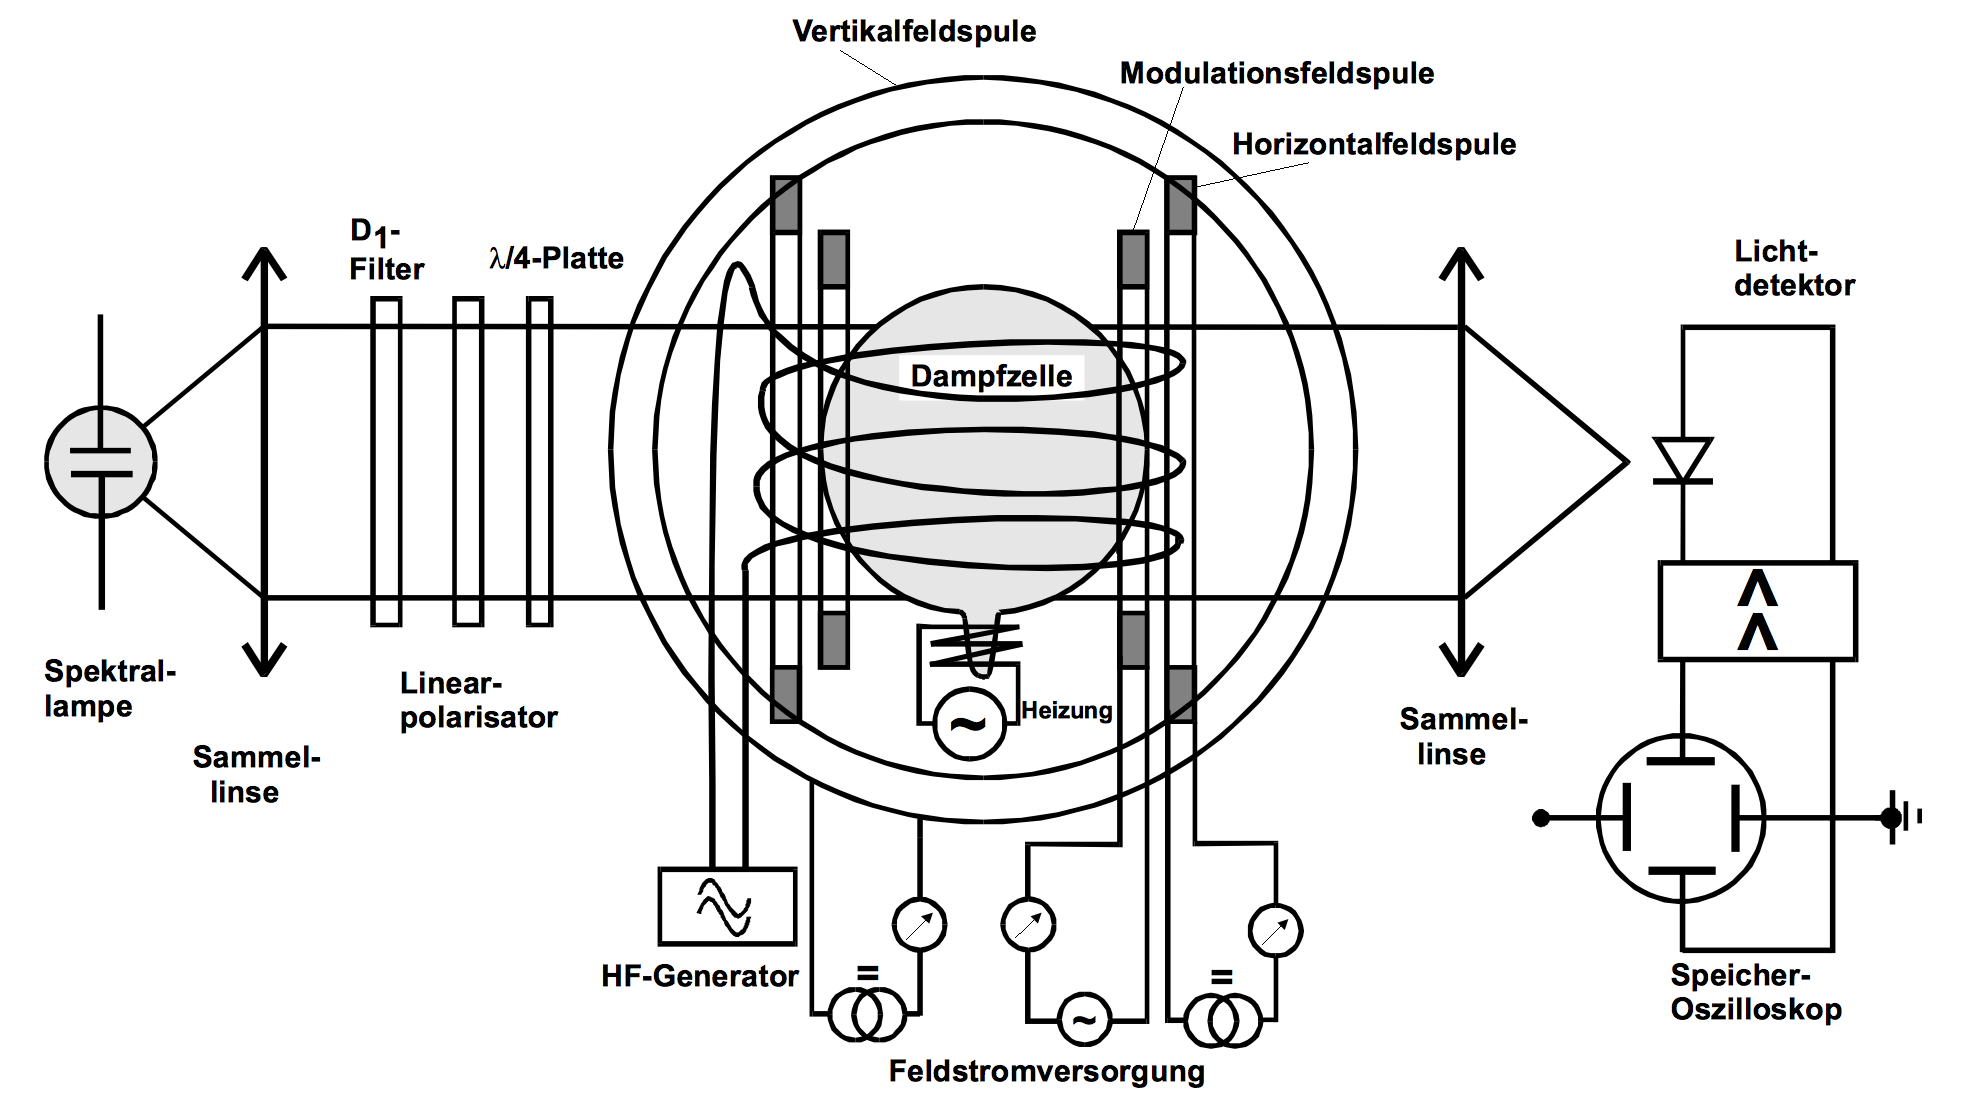
\includegraphics[scale = 0.4]{pictures/aufbau.png}
    \caption{Darstellung des Versuchsaufbaus.\cite{1}}
    \label{fig:aufbau}
\end{figure}
\newline
Das aus der Spektrallampe austretende Licht wird mithilfe einer Sammellinse kollimiert und durch einen $\text{D}_{\su{1}}$-Filter,
welcher nur die zu untersuchende $\text{D}_{\su{1}}$-Linie der Rubidium-Isotope durchlässt, gefiltert.
Der Linearpolarisationsfilter und die $\frac{\lambda}{4}$-Platte im Anschluss sorgen dafür, dass das
aus dem zuvor austretenden Licht zirkular-polarisiertes Licht erzeugt wird. Dieses trifft auf die Dampfzelle, in der
sich die beiden Rubidium-Isotope befinden. Durch das Beheizen der Dampfzelle wird ein optimaler Rubidium-Dampfdruck
eingestellt. Um das durchgetretene Licht auf ein Si-Photoelement zu fokussieren, wird
eine weitere Sammellinse verwendet. An das Photoelement angeschlossen sind ein Linearverstärker
und ein Oszilloskop, mit dem sich Intensitätsänderungen des Lichtes darstellen lassen.

\noindent Um die Dampfzelle herum sind drei Helmholtz-Spulenpaare aufgestellt. Dabei gleicht die eine das wirkende
Erdmagnetfeld aus, wobei die anderen beiden für die Erzeugung der Zeeman-Aufspaltung der
Energieniveaus benötigt werden. Für die Erzeugung der horizontalen Feldern ist eine Sweep-Spule auf ein Horizontalfeld-Spule
gewickelt. \newline
Das durch eine weitere Spule entstandendene RF-Feld dient dazu, dass die Energieübergange abhängig von
der Horizontalfeldstärke sind.
\end{document}
